\documentclass[12pt, twoside]{report}
\usepackage[a4paper,bindingoffset=0.2in,%
            left=0.8in,right=0.8in,top=1.2in,bottom=1.2in,margin=20pt,%
			]{geometry}
\usepackage{inputenc}
\usepackage{graphicx}
\usepackage{fancyhdr}
\usepackage{amsmath}

\fancyhf{}
\renewcommand{\headrulewidth}{0pt}
\fancyhead[RO,LE]{\thepage}
\pagestyle{fancy}

\begin{document}

\begin{figure}
	\centering
	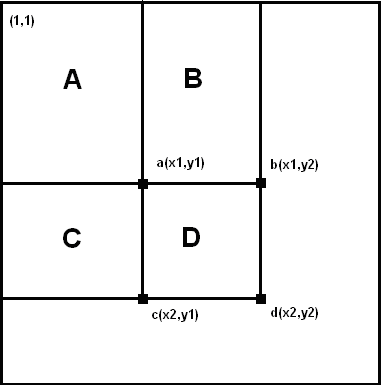
\includegraphics{img/13_1.png}
	\caption{Compute rectangle sum using integral image}
\end{figure}

\par
The use of integral images leads to enormous savings and makes it possible to use Haar
wavelets in a real-time detection system.
\subsubsection{Constructing Weak Classifier}

\par
In Viola’s Framework, ``the AdaBoost learning procedure is used to solve the following
three fundamental problems: 1) learning effective features from a large feature set; 2)
constructing weak classifiers, each of which is based on one of the selected features; and
3) boosting the weak classifiers to construct a strong classifier''. We’ll talk about the
first in this section.Suppose a set of N labeled training examples $(x1, y1), . . . ,(xN , yN )$ is given, where
$yi = {1, −1} $is the label of image $xi$. We also assume a weight$ wi$ is assigned to each example, and how to compute this weight will be given in the next section. $K$ Haar features $F_k, k = 1, 2, . . . K$ can be computed for each image; in Viola’s detection system constructing a weak classifier means determining a feature Fkm, a direction $bm = \{1, −1\}$ and a threshold $f_m$:
\begin{center}
	\begin{equation}
		h_m = \begin{cases}
			+1, & \text{if (F_{k_m} − f_m) b_m > 0} \\
			-1, & \text{otherwise}
		\end{cases}
	\end{equation}	
\end{center}

\par
This simple classifier is called a “stump”. We choose the three parameters $k_m$, $b_k$ and

\newpage

\par
$f_k$ to minimize some objective function, for example weighted classification error. This
optimization can be done in two steps: for each$ Fk$ , find the best$ bk, fk $0and corresponding
weighted error $errk$; then choose $(km, bk, fk)$ which corresponds to the smallest$ errk$.}
\subsubsection*{Boosting Strong Classifier}

\par
AdaBoost iteratively learns a sequence of weak classifiers$ hm$ and constructs a strong one$
HM$ using their linear combination. In each cycle AdaBoost does two things: find the best
linear combination coefficients, and update the sample weights. Both of these tasks are
based on the upper bound on classification error of$ HM$. [74] shows that the bound can be
derived from the following exponential loss function:

\begin{equation}
J(Hm)=\sum  e^{-yiHm(xi)} =\sum e^{-yi \sum amhm(xi)} 
\end{equation}

Given the current strong classifier $H_(m-1)(x)=\sum a_m h_m (x)$ and the newly learned
weak classifier $hM$, the best combining coefficient$ aM$ is the minimizer of the following
optimization problem:

\begin{equation}
a_M=argminJ(H_(m-1)(x)+ah_m(x))
\end{equation}

\begin{equation}
a_M=\log (1-err_M ) /err_M  
\end{equation}

where $err_M$ is the weighted error of $h_M$ defined as

\begin{equation}
err_M=\sum w_i^(M-1)(sgn(h_M(x))-y_i)/2
\end{equation}

Equation (2.17) suggests if the new weak classifier has a good performance (small $err_M$),
we’ll give it a large $a_M$; otherwise it will be assigned a small coefficient.
To update the weight of each training sample, let’s rewrite (2.16) as follows:

\begin{equation}
J(H_m)=\sum e^-y_i \sum a_m h_m (x)
\end{equation}

\newpage

\end{document}
























